\graphicspath{{./Figs/}}

\chapter{Introduction} 
\label{sec:Background}

% What is a MAV


Unmanned aerial vechicles (UAV) are used throughout various industries to conduct missions which are either dangerous, difficult or tedious for humans to perform. The development of technologies and demand for smaller aerial vechicles has lead to the development of Micro aerial vehicles (MAV) \cite{NONAMI2007}. MAV's will become evermore important for both commerical \cite{Liu2014} and millitary \cite{Chaturvedi2019} \cite{Fan2018} use as advancements are made in navigation systems, cooperative control of multiple MAV's, advanced vision systems, embedded computational systems and navigational systems.

%  MAV's do not have a standard guidelines for 
Despite the small size of MAV's there are three main categories these aircraft fit into. These are fixed wings \cite{Stanford2008} \cite{Lasek2001}, rotary wings, flapping wings \cite{Platzer2012} or a combination of these. Due to the small size and Reynolds numbers at which these aircraft operate at (typically around Re=$10^5$ \cite{Huq2009}), insects and other small animals are often studied to understand the flight dynamics which occur for small flying bodies \cite{Liu2009}. The additional complexity to the design of MAV's occurs due to several factors:
\begin{itemize}
  \item Low Reynolds number flight
  \item Small physical dimensions
  \item Structural strength
  \item Reduced stall speed
  \item Low inertia
\end{itemize}

\begin{figure}[H]
  \centering
  % 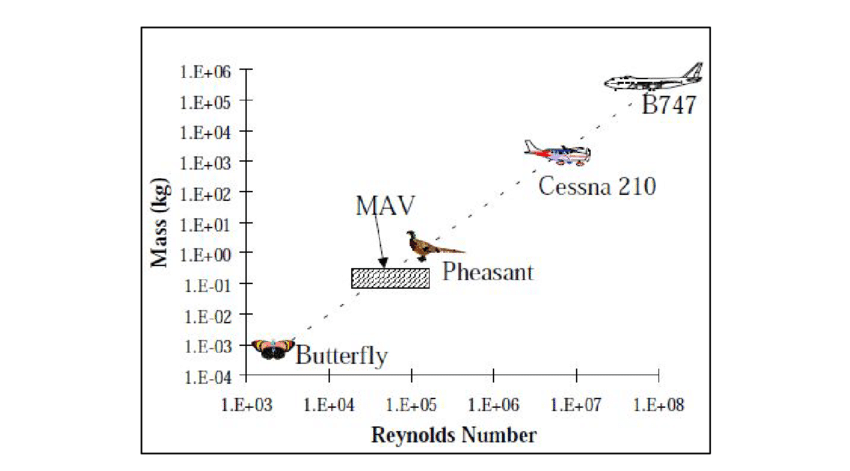
\includegraphics[width=0.8\linewidth]{images/Reynolds.png}
  \caption{MAV speed reynolds number region with respect to flying bodies}
  \label{fig:MAVsizes}
\end{figure}

% \\
With the increased complexity of MAV designs, there has also been increased interest in the reasearch and design of optimized MAV models \cite{Ward2017}. Traditional methods of aircraft design have generally focused on larger aircraft which operate at Reynolds numbers of $10^6$ or more \cite{Raymer2006} \cite{Roskam1989}. There currently does not exist a fully validated, optimised and reliable optimization technique for MAV aircraft. In order to optimize MAV designs, software designed to numerically optimise models are generally based on aerodynamic properties, weights, stability and maneurability \cite{Amadori2012} \cite{Vijayanandh2019} \cite{Radmanesh2014}. The low Reynolds number flight dynamics and non-linear flight dynamics are of particular importance for MAV development \cite{Aboelezz2020} \cite{Aboelezz2021}.The low Reynolds number that MAVs fly at and the influence of an operating propeller on the rest of the MAV is currently unvalidated with physical wind tunnel testing. The main goal of this thesis therefore aims to fill in this gap.\\
\\
Many groups of research have created software to optimize MAV's by using optimization algorthims such as generic algorthims, non-dominating sorting generic algorithms, particle swarm optimization and sequential quadratic optimisation programs.  While some have accounted for low Reynolds numbers \cite{Bronz2009} \cite{Vijayanandh2019} \cite{HASSANALIAN2019}, no optimization techniques accounting for propeller interaction effects currently exist. Many investigations into propeller effects show the propeller has significant effects on wing aerodynamics, both in regards to performance and also stability \cite{Shams2020b} \cite{Chen2022} \cite{Aminaei2018} \cite{Null2005} \cite{Parga2007} \cite{Harikumar2021} \cite{Jana2020}. None have validated these results with physical wind tunnel testing.
\section{Background}
% Intro here

\subsection{Proliferation of MAV's in the Aerospace Landscape}
\label{subsec:ProliferationMAVs}

UAV's have existed for centuries and have been predominately used for survellience and millitary purposes \cite{Aleksander2018}. The recent shift to the miniturization of components, systems and aerial vehicles has already influenced the military sector with several developments underway to reduce visibility of reconansance aircraft and reduce the likelihood of aircraft being detected during missions \cite{Aleksander2018} \cite{Mil2022} \cite{Greenwood2019} \cite{Saytov2022}. What started as a small initial interest in smaller and smarter drones has resulted in exponential growth in the sector \cite{NONAMI2007} \cite{Wang2019} . This coupled together with the growth in camera sensors and computer development, has led to the exponential growth in the capabilities of MAV seen today \cite{Yin2020} \cite{Jackson2016}. Where an inital drone supported only low camera resolution with meagre flight times, today incoporates several systems such as gyrostabilisation, GPS capability with waypoint guidance, beyond the line of vision control, speeds of 70 km/h with a 30 minute flight time and a 20 megapixel camera (DJI Phantom 4) \cite{Peppa2019}.\\

% Look at section \ref{sec:ProliferationMAVs}.

\subsection{Limitations of Current Developed MAV}
\label{subsec:Limitations}
While MAV technology is more accessible and viable to mass market than it has ever been before \cite{Jackson2016}, there is no fully developed and validated way to optimize a MAV for a specified mission \cite{Bronz2009} \cite{HASSANALIAN2019}. Procedures today involve developing a CAD model of the MAV or using software to do so based on aerodynamics. This model is either then run through aerodynamic optimization software and/or tested in a wind tunnel to detemine the main characteristics of the MAV \cite{Paulson2017}. The largest drawback of which is the lack of propeller effects accounted for which are known to have a large effect on aerodynamics and stability \cite{Harikumar2021} \cite{Chinwicharnam2013}. MAV model tests have been conducted with a fixed position propeller \cite{Shams2020b} \cite{Durai2014}. Models are however typically tested without a free-flowing propeller, although these have been included in several aerodynamic software programs and specific tests \cite{Aboelezz2020}. A lack of validation from wind tunnel testing however, means that a full understanding of the effects a propeller has on MAV's has not been achieved. Due to the small size of MAV and the large relative size of the propeller rotor disc compared to both the wing and body size the propeller will significantly affect the stability, noise, overall endurance, performance and power consumption of a given MAV \cite{Shams2020} \cite{Chen2022} \cite{Aminaei2018} \cite{Null2005} \cite{Parga2007} \cite{Harikumar2021} \cite{Jana2020}. 

\subsection{The General Micro Aerial Vechicle}
\label{subsec:GenMAV}
Today the interest, research and development of MAV's is continually increasing, however in order to focus on particular aspects or compare various designs, a "baseline" geometry is required. An example of this is the GENMAV \cite{Stewart2007}. While there are various models which have been tested to determine the main aerodyanmic properties \cite{Stewart2007}\todo{add 2 more examples at least}, none have completed a physical wind tunnel test while accounting for the effects of a powered propeller. Inital GENMAV aerodynamic data was determined by using the vortex-panel method \cite{Stewart2007} and did not involve wind tunnel testing. The effects of propeller induced flow has also been studied for both fixed and free-spinning propellers but currently no data is avaliable for wind tunnel tests of a powered MAV.

\subsection{Optimization Techniques and Validation}
\label{subsec:Optimization}
Many non-standard aircraft designs are evaluated using software in order to analyse aerodynamic characteristics and then optimized through a variety of typical software engineering methods such as the particle swarm method \cite{Gomez2020}. These procedures are typically used as non-standard aircraft designs are more tedious to design and even more complex to setup and test than compared with standard aircraft designs. 


\section{Problem Statement}
\label{ProblemStatement}
MAV's are set to increase the ability to conduct a variety of missions which predominately have military or survellience objectives \cite{Aleksander2018} \cite{Mil2022} \cite{Greenwood2019} \cite{Saytov2022}. In the past troopers would venture on dangerous missions in order to "hopefully" gather useful information while risking their lives \cite{NONAMI2007}. Survellience was conducted initally from hot air balloons, again risking human lives. Later aircraft (mainly helicopters) would be used, costing companies large sums of money in order to survey from a birds eye view \cite{Aleksander2018}. Today drones and UAV's often conduct this work (within certain limits due to range and flight time) \cite{NONAMI2007} \cite{Aleksander2018}. The next major technology jump sees the optimization and miniturization of these aircraft to produce MAV's. \\
\\
MAV's fit a niche and growing market. These aircraft are mainly used for military purposes due to the MAV's main deffering attributes; its smaller size, lower radar visibility and lower noise output. With MAV design becoming one of the fastest growing areas of development in the aerospace industry, there comes an increasing need to have accurate experimental data in order to validate, simulate and model the numerous MAV configurations being investigated. 

% paragraph on impact\significance of MAV
% MAV's

% paragraph on current Limitations

% paragraph on challenge/ main goal 
\section{Objectives}
\label{sec:Objectives}
The objectives of this thesis are as follows:

\begin{enumerate}
  \item To carry out a review of current published literature and determine areas with insufficient or no research avaliable for further development and research.
  \item To design and produce a 3D model of a generic micro aerial vechicle with interchangable empennage.
  \item To conduct wind tunnel testing of the generic micro aerial vechicle model with and without propeller effects.
  \item To analyse data of wind tunnel results and detail the affect that propeller effects have on general micro aerical vehicles.
\end{enumerate}

\section{Outline}
\label{sec:Outline}
An outline of the proposed final submission is listed below, however is subject to change.

\begin{itemize}
  \item Chapter 2: Background and literaure review of relevant topics and reasearch for this thesis
  \item Chapter 3: Proposed setup of analysis
  \item Chapter 4: Implementation
  \item Chapter 5: Results
  \item Chapter 6: Discussion
  \item Chapter 7: Conclusion
\end{itemize}



% \begin{python}[caption=Example computation]
% // Calculate the multiplication of x and y by adding x, y number of times.
% function multiply(x, y):
%   output = 0

%   for i = 0..y:
%     output = output + x

%   return output
% \end{python}
